\begin{enumerate}[label=\thechapter.\arabic*,ref=\thechapter.\theenumi]
    \item The Fourier transform X\brak{j\omega} of the signal\\ $x(t)=\frac{t}{\brak{1+t^2}^2}$ is \rule{1.5cm}{0.15mm}.\hfill{GATE-2022-EC-15}
\begin{enumerate}
	\item[(A)] $\frac{\pi}{2j}\omega e^{-\abs{\omega}}$
	\item[(B)] $\frac{\pi}{2}\omega e^{-\abs{\omega}}$
	\item[(C)] $\frac{\pi}{2j}e^{-\abs{\omega}}$
	\item[(D)] $\frac{\pi}{2}e^{-\abs{\omega}}$
\end{enumerate}

\solution
\iffalse
\let\negmedspace\undefined
\let\negthickspace\undefined
\documentclass[journal,12pt,twocolumn]{IEEEtran}
\usepackage{cite}
\usepackage{amsmath,amssymb,amsfonts,amsthm}
\usepackage{algorithmic}
\usepackage{graphicx}
\usepackage{textcomp}
\usepackage{xcolor}
\usepackage{txfonts}
\usepackage{listings}
\usepackage{enumitem}
\usepackage{mathtools}
\usepackage{gensymb}
\usepackage{comment}
\usepackage[breaklinks=true]{hyperref}
\usepackage{tkz-euclide} 
\usepackage{listings}
\usepackage{gvv}                                        
\def\inputGnumericTable{}                                 
\usepackage[latin1]{inputenc}                                
\usepackage{color}                                            
\usepackage{array}                                            
\usepackage{longtable}                                       
\usepackage{calc}                                             
\usepackage{multirow}                                         
\usepackage{hhline}                                           
\usepackage{ifthen}                                           
\usepackage{lscape}
\usepackage[center]{caption} % center the captions to figure

\newtheorem{theorem}{Theorem}[section]
\newtheorem{problem}{Problem}
\newtheorem{proposition}{Proposition}[section]
\newtheorem{lemma}{Lemma}[section]
\newtheorem{corollary}[theorem]{Corollary}
\newtheorem{example}{Example}[section]
\newtheorem{definition}[problem]{Definition}
\newcommand{\BEQA}{\begin{eqnarray}}
\newcommand{\EEQA}{\end{eqnarray}}
\newcommand{\define}{\stackrel{\triangle}{=}}
\theoremstyle{remark}
\newtheorem{rem}{Remark}
\begin{document}

\newcolumntype{M}[1]{>{\centering\arraybackslash}m{#1}}
\newcolumntype{N}{@{}m{0pt}@{}}

\bibliographystyle{IEEEtran}
\vspace{3cm}

\title{GATE 2022 BM 14 Q} 
\author{ee23btech11223 - Soham Prabhakar More% <-this % stops a space
}
\maketitle
\newpage
\bigskip

\renewcommand{\thefigure}{\theenumi}
\renewcommand{\thetable}{\theenumi}

\bibliographystyle{IEEEtran}

\textbf{Question:} $x\brak{t}$ is a real continuous-time signal whose magnitude frequency response
$\abs{X\brak{j\Omega}}$ is shown below. After sampling $x\brak{t}$ at 100 $rad.s^{-1}$, the spectral point P
is down-converted to \rule{1cm}{0.15mm} $rad.s^{-1}$ in the spectrum of the sampled signal.
\hfill{(GATE 2022 BM 14 Q)}
\begin{figure}[h!]
    \renewcommand\thefigure{1}
    \centering
    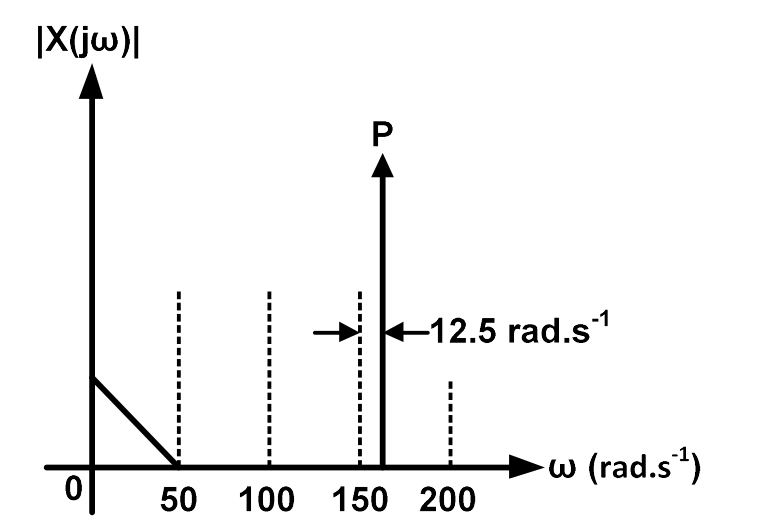
\includegraphics[width=\columnwidth]{2022/BM/14/figs/question.png}
    \caption[short]{Plot of $\abs{X\brak{j\omega}}$}
    \label{fig:2023.bm.14.img1}
\end{figure}

\solution
\fi
\begin{table}[ht]
    \renewcommand\thetable{1}
\begin{tabular}{|c|c|}
    \hline 
    \textbf{Parameter}&\textbf{Description} \\
    \hline
    $w\brak{t}$ & Sampling Function \\
    \hline
	$W\brak{j\omega}$ & Fourier Transform of $w\brak{t}$ \\
    \hline
    $x\brak{t}$ & Input Signal \\
    \hline
    $X\brak{j\omega}$ & Input Signal Frequency Spectrum \\
    \hline
    $x_s\brak{t}$ & Sampled Input Signal \\
    \hline
    $X_s\brak{j\omega}$ & Sampled Signal Frequency Spectrum \\
    \hline
\end{tabular}

\caption{Table of parameters}
\label{Table:1}


\end{table} \\
The sampling function is:
\begin{align}
    w(t) &= \sum_{k = -\infty}^{\infty}\delta\brak{t - \frac{2\pi k}{100}} \\
    W(j\omega) &= 100\sum_{k = -\infty}^{\infty}\delta\brak{j\brak{\omega - 100k}}
\end{align}
then the sampled function: 
\begin{align}
    x_s\brak{t} &= x\brak{t}w\brak{t} \\
    X_s\brak{j\omega} &= X\brak{j\omega} * W\brak{j\omega} \\
    X_s\brak{j\omega} &= \int_{-\infty}^{\infty}X\brak{j\theta}W\brak{j\brak{\omega - \theta}}d\theta \\
    X_s\brak{j\omega} &= 100\sum_{k = -\infty}^{\infty}\int_{-\infty}^{\infty}X\brak{j\theta}\delta\brak{j\brak{\omega - 100k - \theta}}d\theta \\
    X_s\brak{j\omega} &= 100\sum_{k = -\infty}^{\infty}X\brak{j\brak{\omega - 100k}} 
\end{align}
Thus, The down sampled point is at:
\begin{align}
    \omega &= \abs{162.5 - 100k}
\end{align}
where $k$ is the nearest integer to $\frac{162.5}{100}$, which is 2\\
Thus,
\begin{align}
    \omega = 37.5\,rad\,s^{-1}
\end{align}

\begin{figure}[h!]
    \renewcommand\thefigure{2}
    \centering
    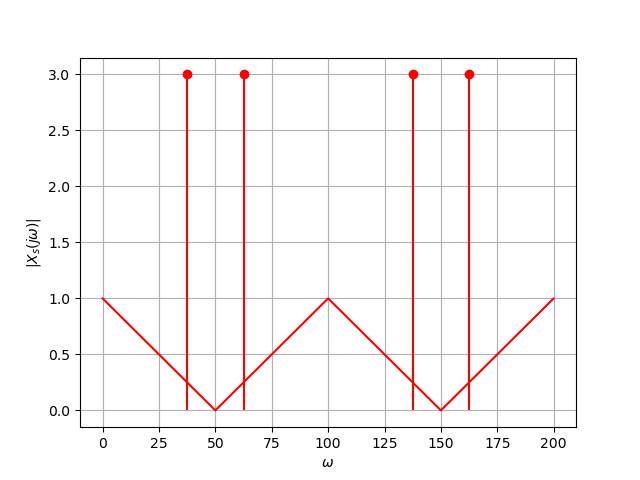
\includegraphics[width=\columnwidth]{2022/BM/14/figs/X_s.png}
    \caption[short]{Plot of $\abs{X_s\brak{j\omega}}$}
    \label{fig:2023.bm.14.img2}
\end{figure}

%\end{document}

\pagebreak

\item For a vector $\bar{x} = [x[0], x[1], \dots, x[7] ]$, the $8$-point discrete Fourier transform (DFT) is denoted by $\bar{X} = \text{DFT}(\bar{x}) = [X[0],X[1],\dots,X[7]]$, where
    \begin{align*}
    X[k] = \sum_{n=0}^{7}x[n]\exp\left(-j\frac{2\pi}{8}nk\right).
    \end{align*} 
    Here $j = \sqrt{-1}$. If $\bar{x} = [1,0,0,0,2,0,0,0]$ and $\bar{y} = \text{DFT}(\text{DFT}(\bar{x}))$, then the value of $y[0]$ is.\hfill{GATE-2022-EC-55}\\
    \solution
    \input{2022/EC/55/55.tex}
    \pagebreak
\item \textbf{Question:} An LTI system is shown in the figure where $$H\brak{s}= \frac{100}{s^2+0.1s+10}$$ The steady state output of the system for an input $x\brak{t}$ is given by $y\brak{t}=a+b\sin{\brak{10t+\theta}}$. The values of $'a'$ and $'b'$ are \\\\
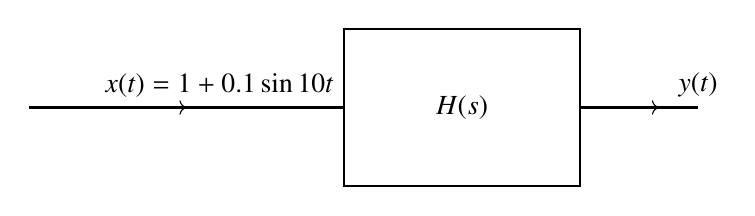
\begin{tikzpicture}
    \draw [thick, draw=black] (-2,-1) -- (2,-1) node[anchor=south east] {$x(t)=1+0.1\sin{\brak{10t}}$};
    \draw [thick,draw=black] (2,0) rectangle (5,-2) ;
    \draw [thick,draw=black] (5,-1) -- (6.5,-1) node[anchor=south] {$y(t)$};
    \draw [->] (-2,-1)--(0,-1);
    \draw [->] (5,-1)--(6,-1);
    \draw (3.5, -1) node[] {$H(s)$};
\end{tikzpicture}\\
\solution 
    \iffalse
\let\negmedspace\undefined
\let\negthickspace\undefined
\documentclass[journal,12pt,twocolumn]{IEEEtran}
\usepackage{cite}
\usepackage{amsmath,amssymb,amsfonts,amsthm}
\usepackage{algorithmic}
\usepackage{graphicx}
\usepackage{textcomp}
\usepackage{xcolor}
\usepackage{txfonts}
\usepackage{listings}
\usepackage{enumitem}
\usepackage{mathtools}
\usepackage{gensymb}
\usepackage{comment}
\usepackage[breaklinks=true]{hyperref}
\usepackage{tkz-euclide} 
\usepackage{listings}
\usepackage{gvv}                                        
\def\inputGnumericTable{}                                 
\usepackage[latin1]{inputenc}                                
\usepackage{color}                                            
\usepackage{array}                                            
\usepackage{longtable}                                       
\usepackage{calc}                                             
\usepackage{multirow}                                         
\usepackage{hhline}                                           
\usepackage{ifthen}                                           
\usepackage{lscape}
\usepackage[center]{caption} % center the captions to figure

\newtheorem{theorem}{Theorem}[section]
\newtheorem{problem}{Problem}
\newtheorem{proposition}{Proposition}[section]
\newtheorem{lemma}{Lemma}[section]
\newtheorem{corollary}[theorem]{Corollary}
\newtheorem{example}{Example}[section]
\newtheorem{definition}[problem]{Definition}
\newcommand{\BEQA}{\begin{eqnarray}}
\newcommand{\EEQA}{\end{eqnarray}}
\newcommand{\define}{\stackrel{\triangle}{=}}
\theoremstyle{remark}
\newtheorem{rem}{Remark}
\begin{document}

\newcolumntype{M}[1]{>{\centering\arraybackslash}m{#1}}
\newcolumntype{N}{@{}m{0pt}@{}}

\bibliographystyle{IEEEtran}
\vspace{3cm}

\title{GATE 2022 BM 14 Q} 
\author{ee23btech11223 - Soham Prabhakar More% <-this % stops a space
}
\maketitle
\newpage
\bigskip

\renewcommand{\thefigure}{\theenumi}
\renewcommand{\thetable}{\theenumi}

\bibliographystyle{IEEEtran}

\textbf{Question:} $x\brak{t}$ is a real continuous-time signal whose magnitude frequency response
$\abs{X\brak{j\Omega}}$ is shown below. After sampling $x\brak{t}$ at 100 $rad.s^{-1}$, the spectral point P
is down-converted to \rule{1cm}{0.15mm} $rad.s^{-1}$ in the spectrum of the sampled signal.
\hfill{(GATE 2022 BM 14 Q)}
\begin{figure}[h!]
    \renewcommand\thefigure{1}
    \centering
    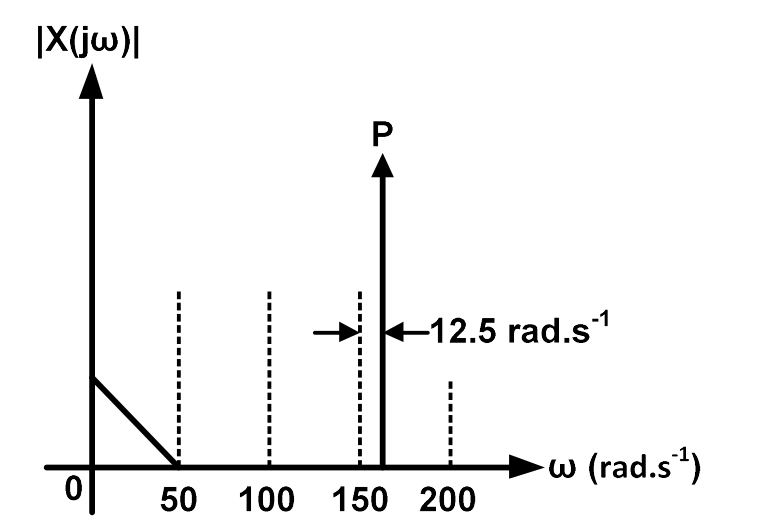
\includegraphics[width=\columnwidth]{2022/BM/14/figs/question.png}
    \caption[short]{Plot of $\abs{X\brak{j\omega}}$}
    \label{fig:2023.bm.14.img1}
\end{figure}

\solution
\fi
\begin{table}[ht]
    \renewcommand\thetable{1}
\begin{tabular}{|c|c|}
    \hline 
    \textbf{Parameter}&\textbf{Description} \\
    \hline
    $w\brak{t}$ & Sampling Function \\
    \hline
	$W\brak{j\omega}$ & Fourier Transform of $w\brak{t}$ \\
    \hline
    $x\brak{t}$ & Input Signal \\
    \hline
    $X\brak{j\omega}$ & Input Signal Frequency Spectrum \\
    \hline
    $x_s\brak{t}$ & Sampled Input Signal \\
    \hline
    $X_s\brak{j\omega}$ & Sampled Signal Frequency Spectrum \\
    \hline
\end{tabular}

\caption{Table of parameters}
\label{Table:1}


\end{table} \\
The sampling function is:
\begin{align}
    w(t) &= \sum_{k = -\infty}^{\infty}\delta\brak{t - \frac{2\pi k}{100}} \\
    W(j\omega) &= 100\sum_{k = -\infty}^{\infty}\delta\brak{j\brak{\omega - 100k}}
\end{align}
then the sampled function: 
\begin{align}
    x_s\brak{t} &= x\brak{t}w\brak{t} \\
    X_s\brak{j\omega} &= X\brak{j\omega} * W\brak{j\omega} \\
    X_s\brak{j\omega} &= \int_{-\infty}^{\infty}X\brak{j\theta}W\brak{j\brak{\omega - \theta}}d\theta \\
    X_s\brak{j\omega} &= 100\sum_{k = -\infty}^{\infty}\int_{-\infty}^{\infty}X\brak{j\theta}\delta\brak{j\brak{\omega - 100k - \theta}}d\theta \\
    X_s\brak{j\omega} &= 100\sum_{k = -\infty}^{\infty}X\brak{j\brak{\omega - 100k}} 
\end{align}
Thus, The down sampled point is at:
\begin{align}
    \omega &= \abs{162.5 - 100k}
\end{align}
where $k$ is the nearest integer to $\frac{162.5}{100}$, which is 2\\
Thus,
\begin{align}
    \omega = 37.5\,rad\,s^{-1}
\end{align}

\begin{figure}[h!]
    \renewcommand\thefigure{2}
    \centering
    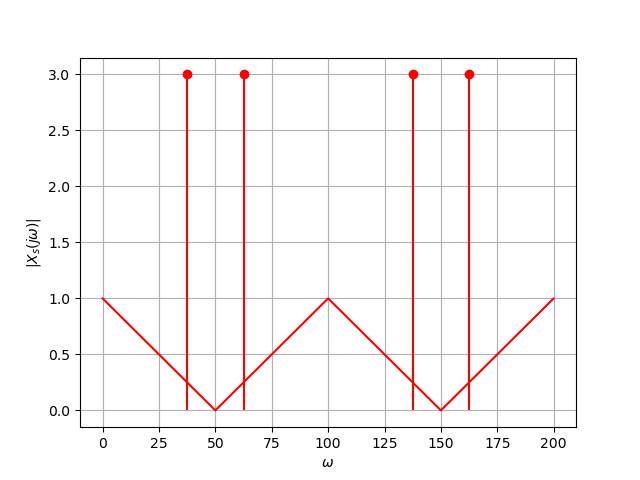
\includegraphics[width=\columnwidth]{2022/BM/14/figs/X_s.png}
    \caption[short]{Plot of $\abs{X_s\brak{j\omega}}$}
    \label{fig:2023.bm.14.img2}
\end{figure}

%\end{document}

\item A periodic function $f(x)$, with period 2, is defined as \\
   \begin{align}   
   f(x) =
   \begin{cases}
    -1-x & -1 \leq x<0 \\
     1-x &  0 <x \leq1 
   \end{cases}
   \end{align} 
   The Fourier series of this function contains \\
\begin{enumerate}[label=\Alph*.]
\item Both $\cos(n\pi x)$ and $sin(n\pi x)$ where n=1,2,3...
\item Only $\sin(n\pi x)$ where n=1,2,3...
\item Only $\cos(n\pi x)$ where n=1,2,3...
\item Only $\cos(2n\pi x)$ where n=1,2,3...  \hfill{GATE IN 2022 }
\end{enumerate} 

\solution
\input{2022/IN/13/g13.tex}
\item  A Simple closed path C in the Complex Plane is shown in the figure.
 \begin{align*}
        \oint_C \frac{2^z}{z^2-1}dz=-\jmath \pi A
 \end{align*}
 Where $\jmath=\sqrt{-1}$, Then find the value of A is \rule{1cm}{0.15mm}(Rounded of to two decimals)
\begin{figure}[h!]
    \centering
    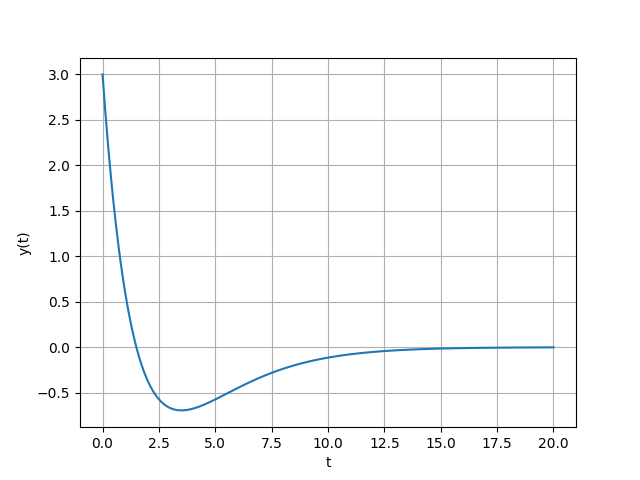
\includegraphics[width = \columnwidth]{2022/EC/32/figs/fig1.png}
\end{figure}
\hfill{(GATE 2022 EC)}\\
\solution 
\input{2022/EC/32/EC_32.tex}
\pagebreak
\item Consider the wave elevation spectrum $S_{\eta \eta}(\omega)$ as shown in the figure. Then, the significant wave height is \underline{\hspace{3cm}} m.
\begin{figure}[H]
    \centering
    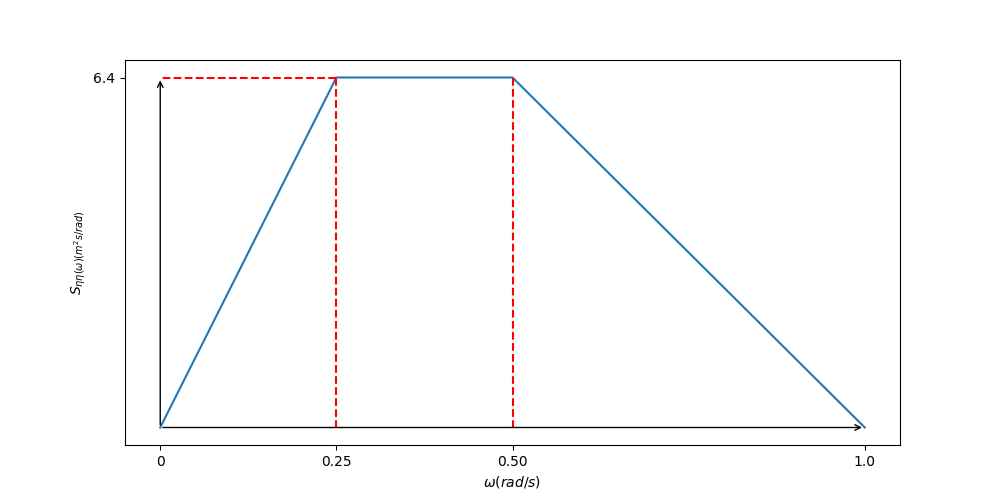
\includegraphics[width=\columnwidth]{2022/NM/40/figs/qfig.png}
    \caption{Wave Elevation Spectrum}
    \label{fig: GATE22NM40.1}
\end{figure}

\begin{enumerate}[label=(\Alph*)]
\item 2
\item 4
\item 6
\item 8
\end{enumerate}
\hfill{GATE NM 2022} \\
\solution \\
\iffalse
\let\negmedspace\undefined
\let\negthickspace\undefined

\documentclass[journal,12pt,onecolumn]{IEEEtran}

\usepackage{cite}
\usepackage{amsmath,amssymb,amsfonts,amsthm}
\usepackage{graphicx}
\usepackage{textcomp}
\usepackage{xcolor}
\usepackage{txfonts}
\usepackage{listings}
\usepackage{enumitem}
\usepackage{mathtools}
\usepackage{gensymb}
\usepackage[breaklinks=true]{hyperref}
\usepackage{tkz-euclide}
\usepackage{listings}
\usepackage{float}

\newtheorem{theorem}{Theorem}[section]
\newtheorem{problem}{Problem}
\newtheorem{proposition}{Proposition}[section]
\newtheorem{lemma}{Lemma}[section]
\newtheorem{corollary}[theorem]{Corollary}
\newtheorem{example}{Example}[section]
\newtheorem{definition}[problem]{Definition}
\newcommand{\BEQA}{\begin{eqnarray}}
\newcommand{\EEQA}{\end{eqnarray}}
\newcommand{\define}{\stackrel{\triangle}{=}}
\theoremstyle{remark}
\newtheorem{rem}{Remark}

\begin{document}

\providecommand{\pr}[1]{\ensuremath{\Pr\left(#1\right)}}
\providecommand{\prt}[2]{\ensuremath{p_{#1}^{\left(#2\right)} }}
\providecommand{\qfunc}[1]{\ensuremath{Q\left(#1\right)}}
\providecommand{\sbrak}[1]{\ensuremath{{}\left[#1\right]}}
\providecommand{\lsbrak}[1]{\ensuremath{{}\left[#1\right.}}
\providecommand{\rsbrak}[1]{\ensuremath{{}\left.#1\right]}}
\providecommand{\brak}[1]{\ensuremath{\left(#1\right)}}
\providecommand{\lbrak}[1]{\ensuremath{\left(#1\right.}}
\providecommand{\rbrak}[1]{\ensuremath{\left.#1\right)}}
\providecommand{\cbrak}[1]{\ensuremath{\left\{#1\right\}}}
\providecommand{\lcbrak}[1]{\ensuremath{\left\{#1\right.}}
\providecommand{\rcbrak}[1]{\ensuremath{\left.#1\right\}}}
\newcommand{\sgn}{\mathop{\mathrm{sgn}}}
\providecommand{\abs}[1]{\left\vert#1\right\vert}
\providecommand{\res}[1]{\Res\displaylimits_{#1}} 
\providecommand{\norm}[1]{\left\lVert#1\right\rVert}
\providecommand{\mtx}[1]{\mathbf{#1}}
\providecommand{\mean}[1]{E\left[ #1 \right]}
\providecommand{\cond}[2]{#1\middle|#2}
\providecommand{\fourier}{\overset{\mathcal{F}}{ \rightleftharpoons}}
\newenvironment{amatrix}[1]{%
  \left(\begin{array}{@{}*{#1}{c}|c@{}}
}{%
  \end{array}\right)
}
\newcommand{\solution}{\noindent \textbf{Solution: }}
\newcommand{\cosec}{\,\text{cosec}\,}
\providecommand{\dec}[2]{\ensuremath{\overset{#1}{\underset{#2}{\gtrless}}}}
\newcommand{\myvec}[1]{\ensuremath{\begin{pmatrix}#1\end{pmatrix}}}
\newcommand{\mydet}[1]{\ensuremath{\begin{vmatrix}#1\end{vmatrix}}}
\newcommand{\myaugvec}[2]{\ensuremath{\begin{amatrix}{#1}#2\end{amatrix}}}
\providecommand{\rank}{\text{rank}}
\providecommand{\pr}[1]{\ensuremath{\Pr\left(#1\right)}}
\providecommand{\qfunc}[1]{\ensuremath{Q\left(#1\right)}}
	\newcommand*{\permcomb}[4][0mu]{{{}^{#3}\mkern#1#2_{#4}}}
\newcommand*{\perm}[1][-3mu]{\permcomb[#1]{P}}
\newcommand*{\comb}[1][-1mu]{\permcomb[#1]{C}}
\providecommand{\qfunc}[1]{\ensuremath{Q\left(#1\right)}}
\providecommand{\gauss}[2]{\mathcal{N}\ensuremath{\left(#1,#2\right)}}
\providecommand{\diff}[2]{\ensuremath{\frac{d{#1}}{d{#2}}}}
\providecommand{\myceil}[1]{\left \lceil #1 \right \rceil }
\newcommand\figref{Fig.~\ref}
\newcommand\tabref{Table~\ref}
\newcommand{\sinc}{\,\text{sinc}\,}
\newcommand{\rect}{\,\text{rect}\,}
\let\vec\mathbf
\bibliographystyle{IEEEtran}
\bigskip
Q: Consider the wave elevation spectrum $S_{\eta \eta}(\omega)$ as shown in the figure. Then, the significant wave height is \underline{\hspace{3cm}} m.
\begin{figure}[H]
    \centering
    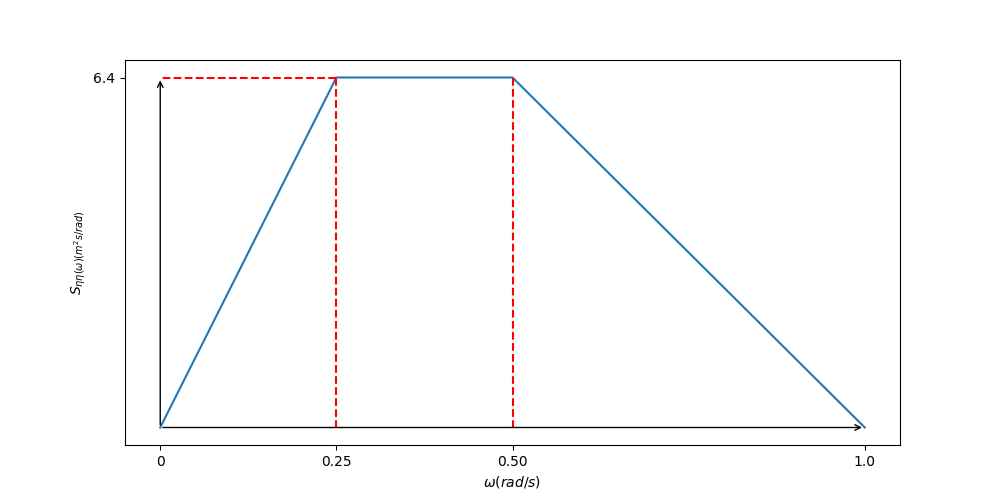
\includegraphics[width=\columnwidth]{2022/NM/40/figs/qfig.png}
    \caption{Wave Elevation Spectrum}
    \label{fig: GATE22NM40.1}
\end{figure}

\begin{enumerate}[label=(\Alph*)]
\item 2
\item 4
\item 6
\item 8
\end{enumerate}
\hfill{GATE NM 2022}


\solution
\fi
Given:
\begin{align}
S_{\eta \eta}(\omega)(m^2s/rad) = 
\begin{cases}
  25.6\omega   & \text{if } \omega \in [0,0.25] \\
  6.4  & \text{if } \omega \in (0.25,0.50] \\
  12.8\omega-12.8  & \text{if } \omega \in (0.50,1.0] \\
  0  & o.w \\
\end{cases}
\end{align}
In terms of f:
\begin{align}
S_{\eta \eta}(f)(m^2s) = 
\begin{cases}
  51.2\pi f   & \text{if } f \in [0,\frac{\pi}{2}] \\
  6.4  & \text{if } f \in (\frac{\pi}{2},\pi] \\
  25.6\pi f-12.8  & \text{if } f \in (\pi,2\pi] \\
  0 & o.w \\
\end{cases} \label{eq: GATE22NM40.1}
\end{align}
Significant Wave Height:
\begin{align}
H_s &= 4 \sqrt{\int_{0}^{\infty} S(f)df}
\end{align}
From \eqref{eq: GATE22NM40.1}
\begin{align}
H_s &= 4 \sqrt{\int_{0}^{\frac{\pi}{2}} 51.2\pi fdf + \int_{\frac{\pi}{2}}^{\pi} 6.4df + \int_{\pi}^{2\pi} (25.6\pi f-12.8)df} \\
&= 4 \sqrt{0.8 +1.6 +1.6} \\
\therefore H_s &= 8
\end{align}
Hence the answer is option (D).
%table
%\begin{table}[!h]
%\begin{tabular}[12pt]{ |c| c|c|}
    \hline
    \textbf{Parameter} & \textbf{Description} & \textbf{Value}\\ 
    \hline
    $y^{''} -  4y^{'} -12y = 3e^{5x}$ & Differential equation & none\\
    \hline
    $y\brak{x}$ &Solution of  differential equation & $y(0)=\frac{18}{7}$\\
    \hline
    $y^{'}\brak{x}$ & First order derivative of solution of differential equation & $y^{'}\brak{0}=\frac{-1}{7}$\\
    \hline
     \end{tabular} 

%\caption{Input Parameter Table}
%\label{tab:q.no.1}
%\end{table}

%figure
%\begin{figure}[H]
%    \centering
%    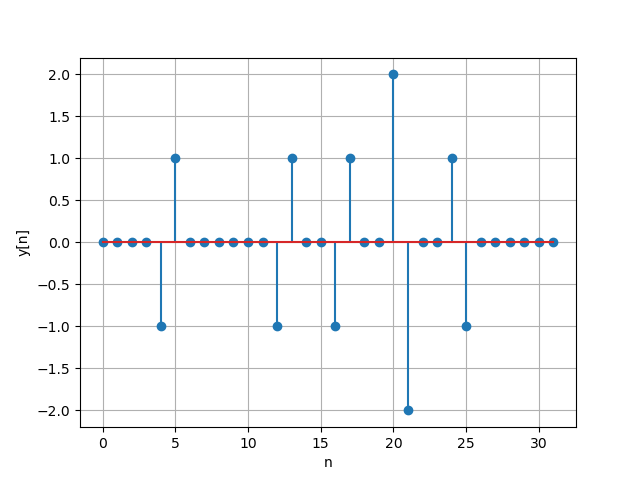
\includegraphics[width=\columnwidth]{./figs/fig.png}
%    \caption{caption}
%    \label{fig: q.no.1}
%\end{figure}

%\end{document}

\pagebreak
\end{enumerate}
